\title{Объектно-центричное представление мира агента в обучении с подкреплением}

\author{%
    \textbf{Студент:}~Ярослав Ивченков \inst{1} \\
    \textbf{Научный руководитель:}~Матвеев И. А.,~д.т.н. \inst{1} 
}

\institute[shortinst]{%
    \inst{1} Московский Физико-Технический Институт \samelineand 
    \inst{2} Научно-Исследовательский Институт Искусственного Интеллекта (AIRI)
}

\titlegraphic{
    % \begin{figure}
    %     \begin{subfigure}{.8\textwidth}
    %         \centering
    %         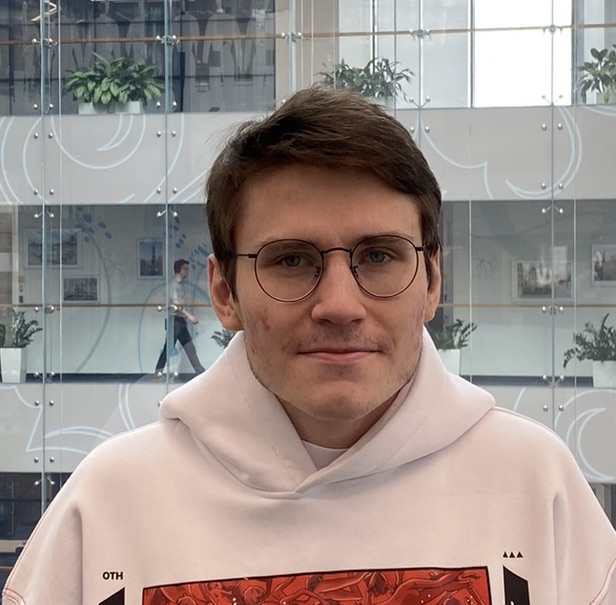
\includegraphics[height=2cm]{images/authors/ivchenkov_yaroslav.jpeg}
    %         \centering
    %         \hspace{2em}
    %         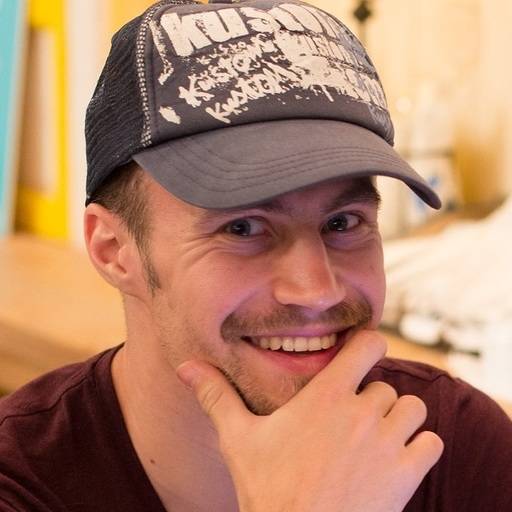
\includegraphics[height=2cm]{images/authors/panov_aleksandr.png}
    %     \end{subfigure}
    % \end{figure}
    \begin{figure}
        \begin{subfigure}{.45\textwidth}
            \raggedleft
            
\includegraphics[height=1.5cm]{images/logos/mipt.png}
        \end{subfigure}
        \begin{subfigure}{.45\textwidth}
            \raggedright
            
\includegraphics[height=0.8cm]{images/logos/airi_dark.png}
        \end{subfigure}
    \end{figure}
    %\parbox[c]{3cm}{
\includegraphics[height=2cm]{images/logos/mipt.png}}
    %\hspace{0.75cm}%
    %\parbox[c]{4cm}{
\includegraphics[height=1.15cm]{images/logos/airi_dark.png}}
}

\setbeamercolor{page number in head/foot}{fg=background canvas.bg}
\begin{frame}
\titlepage
\end{frame}
\note{Hello, my name is Yaroslav and I'm presenting Factorized World Models for Learning Causal Relationships. This is joint work with Artem Zholus from Moscow Institute of Physics and Technology and Aleksandr Panov from Artificial Intelligence Research Institute.\\
\textasciitilde 15s}